%----------------------------------------------------------------------------------------
%    PACKAGES AND THEMES
%----------------------------------------------------------------------------------------

\documentclass[aspectratio=169,xcolor=dvipsnames]{beamer}
\usetheme{SimpleDarkBlue}
\usepackage{tikz}
\usetikzlibrary{arrows.meta,decorations.pathmorphing,positioning}
\usepackage{graphicx}
\usepackage{pdfpages}
\usepackage{graphicx} % Allows including images
\usepackage{booktabs} % Allows the use of \toprule, \midrule and \bottomrule in tables
\usepackage{hyperref}
\usepackage{algorithmicx}
\usepackage{algorithm2e}
\usepackage{subcaption} 
%----------------------------------------------------------------------------------------
%    TITLE PAGE
%----------------------------------------------------------------------------------------

\title{Improving Group Fairness in Knowledge Distillation
via Laplace Approximation of Early Exits}
% \subtitle{Experiments on Confidence Scoring}

\author{ Edvin 24V0074 \and Sagar 24D0367 }
% Kapil 210100079 }

\institute
{
    CS 769 \\
    Optimization in Machine Learning % Your institution for the title page
}
\date{2 May 2025} % Date, can be changed to a custom date

%----------------------------------------------------------------------------------------
%    PRESENTATION SLIDES
%----------------------------------------------------------------------------------------

\begin{document}

\begin{frame}
    % Print the title page as the first slide
    \titlepage
\end{frame}

\begin{frame}{Overview}
    % Throughout your presentation, if you choose to use \section{} and \subsection{} commands, these will automatically be printed on this slide as an overview of your presentation
    \tableofcontents
\end{frame}

\section{Recap from Seminar}

\begin{frame}{Recap from Seminar}
    \begin{itemize}
        \item<1-> Knowledge Distillation as an effective way to distill knowledge from teacher to student% 
        \item<2-> Teacher Provides "Soft Targets"
        \item<3-> Loss: kl divergence $+$ cross-entropy
        \item<4-> Student model relies on spurious correlations
        \item<5-> Student's early Layers overconfident on hard instances
        \item<6-> DEDIER loss
        \[ \mathcal{L}_{student} =
          \sum_{D_w}^{} (1- \lambda) \cdot l_{ce} 
          + \lambda \cdot \textbf{wt} \cdot l_{kd} \] 
          where \(\bf{wt} = \exp^{\beta.\bf{cm}.\alpha} \) and \(\bf{cm(p)} = p_{max} - \max_{p_k \in \bf{p} - p_{max}} p_k \) 
    \end{itemize}
\end{frame}

\begin{frame}{Recap from Seminar}
    \begin{itemize}
        \item<1-> Two alternate approaches for estimating uncertainity in prediction in early exit layers.
        \item<2-> \cite{meronen_fixing_2023} used Laplace approximation for bayesian posterior at exit layer.
        \item<3-> \cite{jazbec_early-exit_2024} used AVCS based on Predictive-likelihood ratio to get confidence intervals for predictions.
        \item<4-> Experiment: Laplace Approximation based uncertainity estimate to reweight both the losses.
    \end{itemize}
\end{frame}

\begin{frame}{Recap from Seminar}

    \only<1>{
        \begin{figure}
            \caption{}
            \centering
            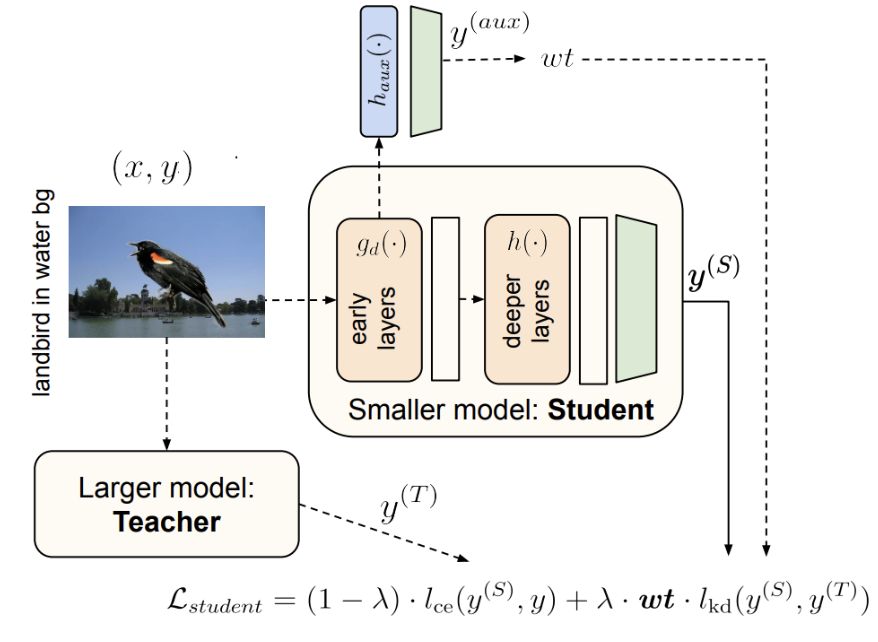
\includegraphics[width=0.6\textwidth]{figs/fig_4.png}
        \end{figure}
    }

    \only<2>{
        \begin{figure}
            \caption{}
            \centering
            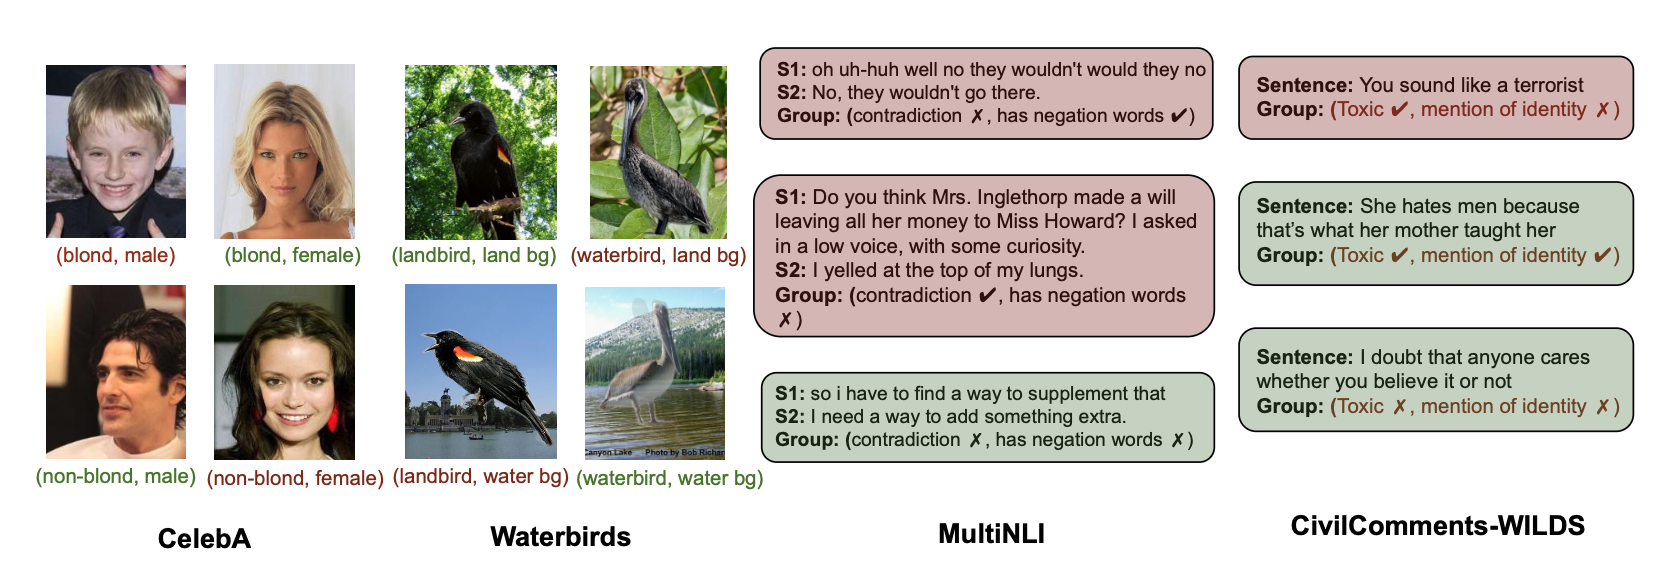
\includegraphics[width=\textwidth]{figs/fig_6.png}
        \end{figure}
    }

    \only<3>{
        \begin{figure}
            \caption{}
            \centering
            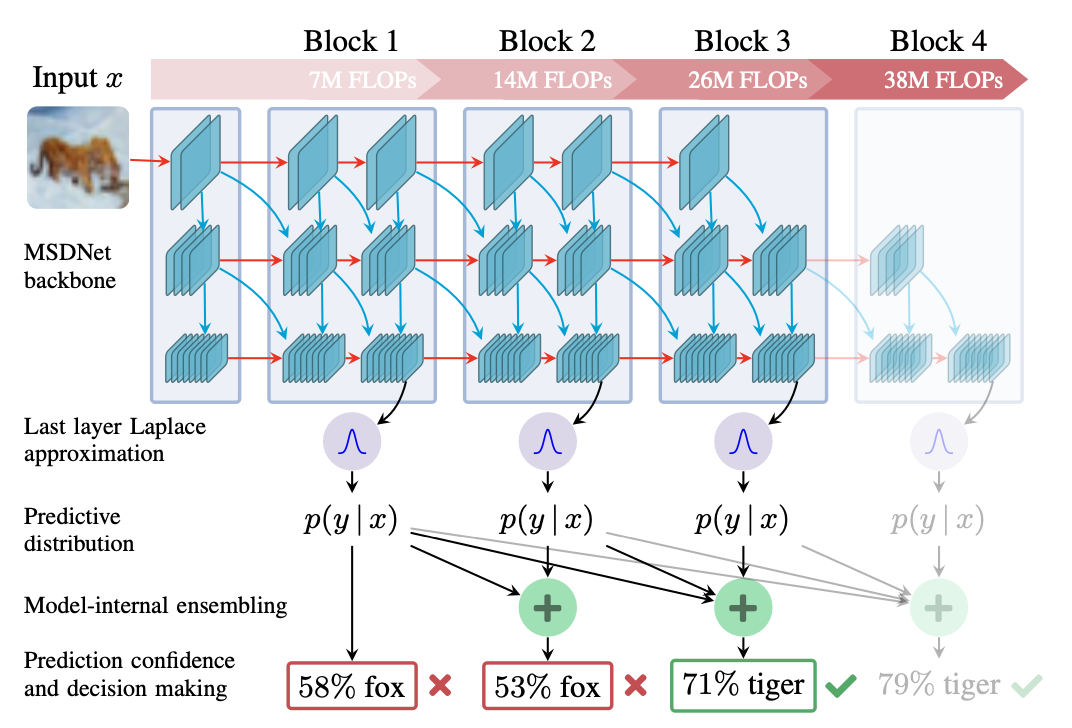
\includegraphics[width=0.4\linewidth]{figs/Screenshot 2025-04-08 at 15.02.28.png}
        \end{figure}
    }

    \only<4>{
        \begin{figure}
            \caption{}
            \centering
            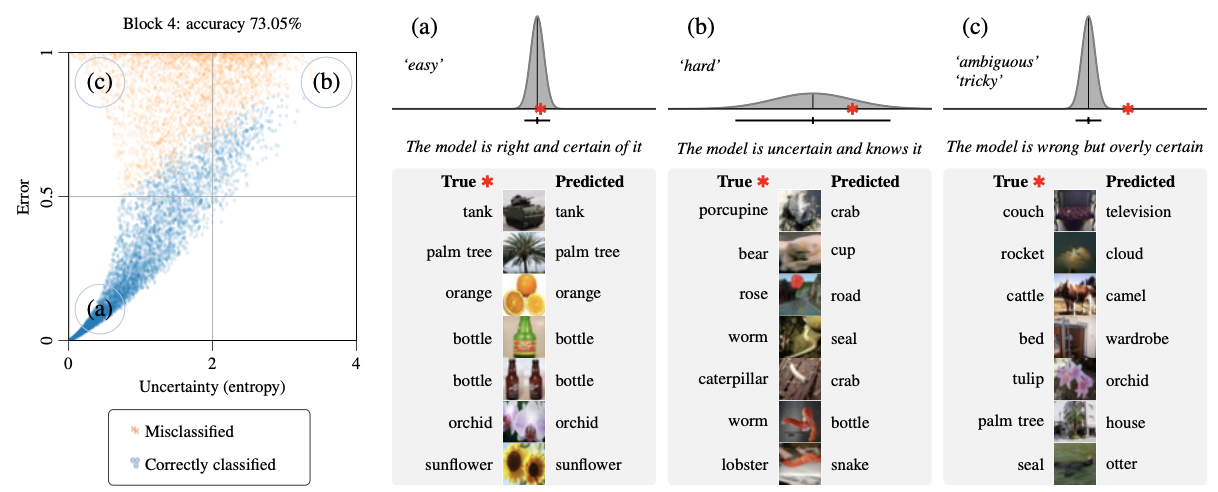
\includegraphics[width=0.7\linewidth]{figs/Screenshot 2025-04-08 at 15.14.46.png}
        \end{figure}
    }
\end{frame}

\begin{frame}{Recap from Seminar}
    \begin{itemize}
        \item<1-> 
        \[
        p(\boldsymbol{\theta} \mid \mathcal{D}_{\text{train}})
        = \frac{p(\mathcal{D}_{\text{train}} \mid \boldsymbol{\theta}) \, p(\boldsymbol{\theta})}{\int_{\boldsymbol{\theta}} p(\mathcal{D}_{\text{train}}, \boldsymbol{\theta}) \, d\boldsymbol{\theta}}
        = \frac{\text{[likelihood]} \times \text{[prior]}}{\text{[model evidence]}}
    \]
        \item<2-> MAP estimate can be found by maximising the unnormalised posterior:
        \[
        \hat{\boldsymbol{\theta}} = \arg\max_{\boldsymbol{\theta}} \log p(\mathcal{D}_{\text{train}} \mid \boldsymbol{\theta}) + \log p(\boldsymbol{\theta})
              \]
        \item<3-> Gaussian distribution via laplace approximation
        \[
        p(\hat{\mathbf{z}}_i \mid \mathbf{x}_i) = \mathcal{N}(\hat{\mathbf{W}}_{\text{MAP}}^\top \hat{\boldsymbol{\phi}}_i, \, (\hat{\boldsymbol{\phi}}_i^\top \mathbf{V} \hat{\boldsymbol{\phi}}_i) \mathbf{U})
        \]
        \[
            \mathbf{V}^{-1} \otimes \mathbf{U}^{-1} = \mathbf{H}^{-1}
        \] where $H$ is 
        \[ \mathbf{H} := - \nabla_{\boldsymbol{\theta}}^2 \log p(\boldsymbol{\theta} | \mathcal{D}) \Big|_{\boldsymbol{\theta}_{\text{MAP}}} \]
        \item<4-> Samples
        \[
         \hat{\mathbf{z}}_i^{(l)} = \hat{\mathbf{W}}_{\text{MAP}}^\top \hat{\boldsymbol{\phi}}_i + (\hat{\boldsymbol{\phi}}_i^\top \mathbf{V} \hat{\boldsymbol{\phi}}_i)^{\frac{1}{2}} (\mathbf{L} \mathbf{g}^{(l)})
        \]
        {\footnotesize \quad $\mathbf{g}^{(l)} \sim \mathcal{N}(0, \mathbf{I})$ and $\mathbf{L}$ is the Cholesky factor of $\mathbf{U}$}
    \end{itemize}
\end{frame}

\section{Experiments And Results}

\begin{frame}{Experiments And Results}

    \only<1>{
        \begin{itemize}
            \item The MultiNLI dataset \cite{williams2018broad} was used.
            \item Determine if premise entails, contradicts, or is neutral given a hypothesis.
            \item Major Diffrences with DEDIER: The auxiliary reweighting is done in every epoch, as student trained for five epochs.
            \item The auxiliary network used is a simple, single layer network.
            \item Models Used
            \begin{itemize}
                \item \textbf{Teacher model:} \texttt{bert-base-uncased} (12-layer BERT, hidden size 768)
                \item \textbf{Student model:} \texttt{distilbert-base-uncased} (6-layer DistilBERT, hidden size 768)
                \item \textbf{Auxiliary network:} One-layer linear classifier trained on the students third layer.
            \end{itemize}
        \end{itemize}
    }

    \only<2>{
       \begin{itemize}
        \item Hyperparameters
        \begin{itemize}
            \item \textbf{Teacher fine-tuning}
            \begin{itemize}
                \item Epochs: $E_T = 3$
                \item Learning rate: $2 \times 10^{-5}$
                \item Optimizer: AdamW
            \end{itemize}
            \item \textbf{Student training}
            \begin{itemize}
                \item Epochs: $E_S = 5$
                \item Learning rate: $2 \times 10^{-5}$
                \item Optimizer: AdamW
                \item Distillation temperature: $\tau = 2.0$
            \end{itemize}
        \end{itemize}

        \item Training and Evaluation
        \begin{itemize}
            \item Batch size: 16
            \item Dataset: MultiNLI (via HuggingFace \texttt{datasets})
            \item Evaluation: Accuracy and per-group performance (negation vs. non-negation)
            \item Tokenization: \texttt{bert-base-uncased} tokenizer with padding and truncation
            \item Learning rate scheduler: Linear schedule with warm-up
        \end{itemize}

       \end{itemize}
    }

    % \only<3>{
    %     \begin{algorithm}
    %         \caption{DeDiER with auxiliary projector and Laplace margins on MultiNLI}
    %         \textbf{Inputs:} Teacher $T$, Student $S$, Projector $h_{\text{aux}}$, dataset $\mathcal{D}$, hyperparameters $\alpha$, $\beta$, number of epochs $E$.
            
    %         \begin{algorithmic}[1]
    %         \STATE Pre-train or load teacher model $T$ on $\mathcal{D}$
    %         \STATE Initialize student $S$ and auxiliary projector $h_{\text{aux}}$
    %         \FOR{$e = 1$ to $E$}
    %             \FOR{each minibatch $(x, y, m)$ from $\mathcal{D}$}
    %                 \STATE Compute features $\phi = T_{\text{BERT}}(x)$ (CLS embedding)
    %                 \STATE Train projector $h_{\text{aux}}$ using cross-entropy on $(\phi, y)$
            
    %                 \STATE Compute logits $z^{(\text{aux})} = h_{\text{aux}}(\phi)$
    %                 \STATE Compute Laplace covariance matrix $\Sigma$ using $h_{\text{aux}}$ and $\phi$
    %                 \STATE Sample predictive distribution: $p = \mathbb{E}_{z \sim \mathcal{N}(z^{(\text{aux})}, \Sigma)} [\text{softmax}(z)]$
    %                 \STATE Compute entropy margin: $\mathcal{H}(p) = -\sum_j p_j \log p_j$
    %                 \STATE Compute weight $w = \exp(\beta \cdot \mathcal{H}(p)^\alpha)$
            
    %                 \STATE Get teacher logits $z^{(T)} = T(x)$
    %                 \STATE Get student logits $z^{(S)} = S(x)$
    %                 \STATE Compute KD loss: $\mathcal{L}_{\text{KD}} = \text{KLDiv}(z^{(S)}, z^{(T)})$
    %                 \STATE Compute CE loss: $\mathcal{L}_{\text{CE}} = \text{CE}(z^{(S)}, y)$
    %                 \STATE Total loss: $\mathcal{L} = w \cdot \mathcal{L}_{\text{KD}} + \mathcal{L}_{\text{CE}}$
    %                 \STATE Update student parameters via backprop on $\mathcal{L}$
    %             \ENDFOR
    %         \ENDFOR
    %         \STATE Save final student model and evaluate on test set
    %         \end{algorithmic}
    %         \end{algorithm}
    % }

    
    \only<3>{
        \begin{table}[h!]
            \centering
            \begin{tabular}{|l|c|c|c|c|}
            \hline
            Metric                          & Teacher & Student (Aux layer 3) & Student (Aux layer 6) & Group \\
            \hline
            Average Accuracy                & 0.845   & 0.835 & 0.832  & All   \\
            \hline
            % Add your other data rows here, ensuring 5 columns per row
            % Example:
            % Another Metric                & value1  & value2 & value3 & GroupX \\
            % \hline
            \end{tabular}
            \caption{Results of Dedier with Laplace}
            \label{fig:results table}
        \end{table}
    }
    
    \only<4>{
        \begin{table}[h!]
            \centering
            \begin{tabular}{|l|c|c|}
            \hline
            Metric             & Teacher & Student \\
            \hline
            Final Test Accuracy & 0.841   & 0.830   \\
            \hline
            \end{tabular}
            \caption{Original DEDIER performance with same teacher}
            \label{fig:enter-label}
        \end{table}
    }

    \only<5>{
        \begin{figure}[]
            \centering
            \begin{subfigure}[t]{0.45\linewidth}
                \centering
                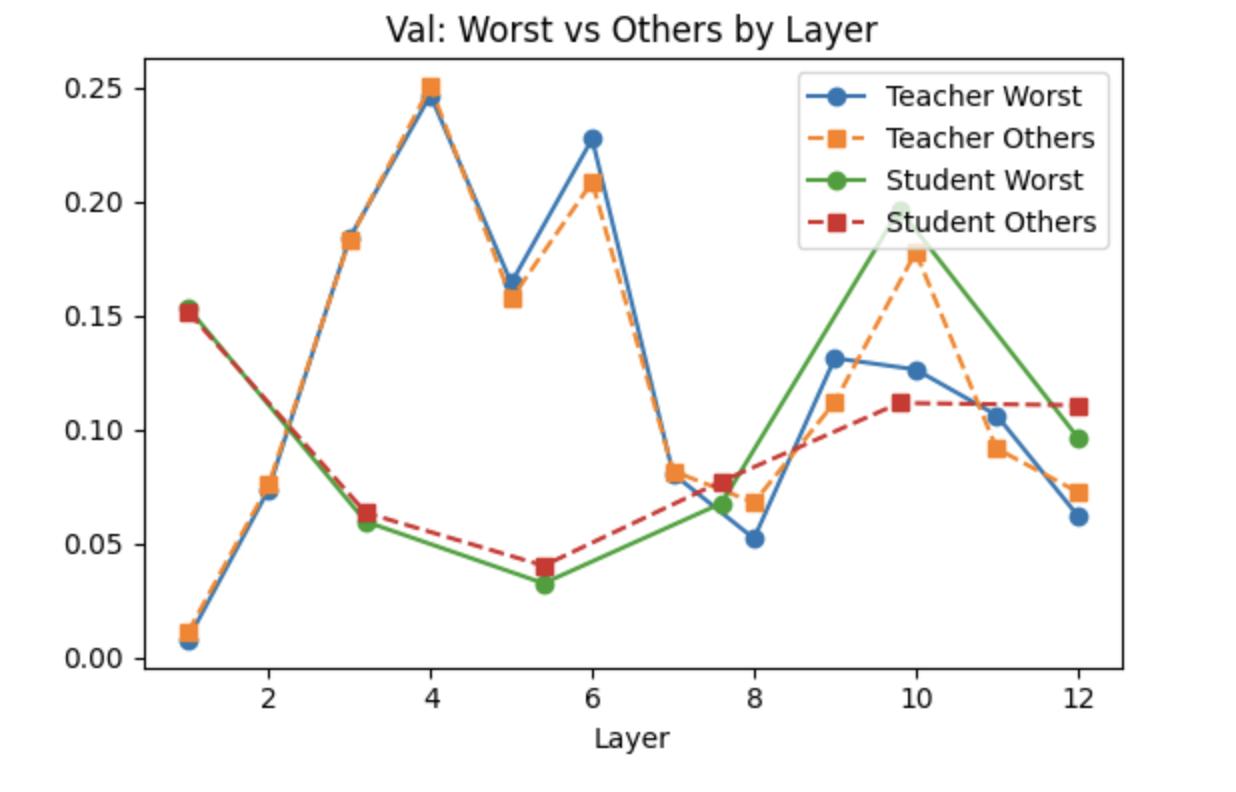
\includegraphics[width=\linewidth]{figs/aux_3_layer.png}
                \caption{Auxiliary network on layer 3}
                \label{fig:aux3}
            \end{subfigure}
            \hfill
            \begin{subfigure}[t]{0.45\linewidth}
                \centering
                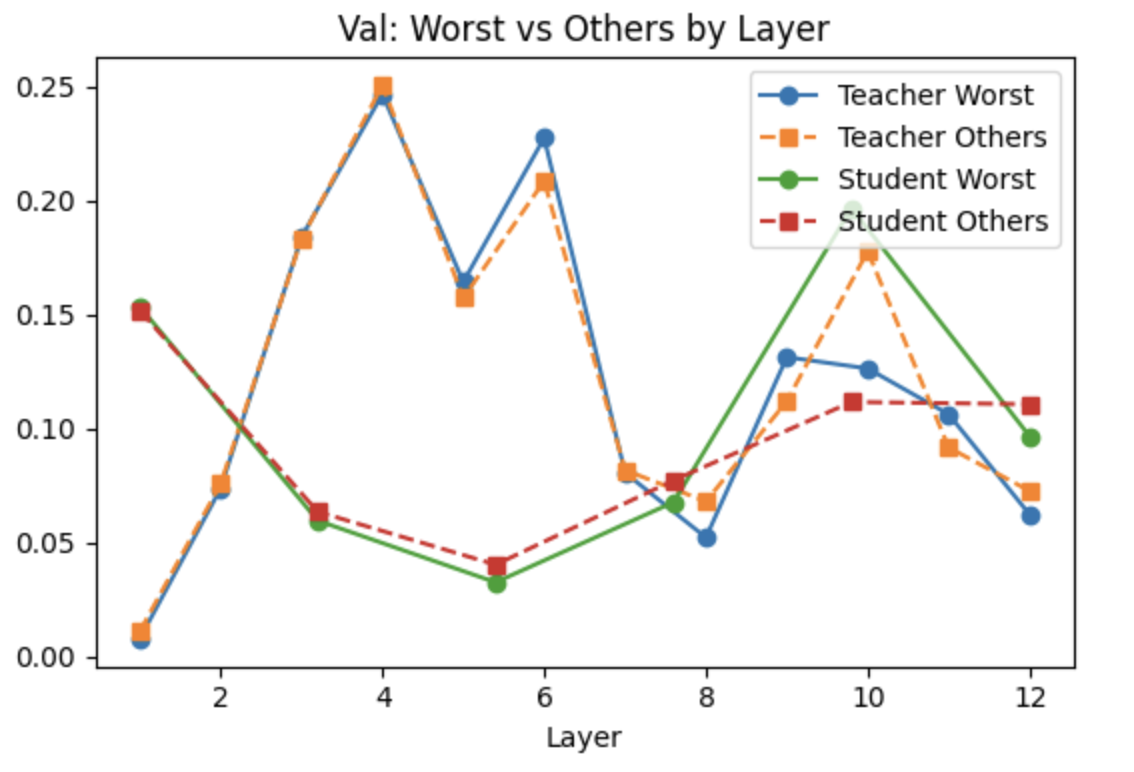
\includegraphics[width=\linewidth]{figs/aux_6_layer.png}
                \caption{Auxiliary network on layer 6 (last layer)}
                \label{fig:aux6}
            \end{subfigure}
            \caption{Confidence margins per layer on worst group predictions and all predictions}
            \label{fig:layer-prediction}
        \end{figure}
    }

    \only<6>{
        \begin{figure}[]
            \centering
            \begin{subfigure}[t]{0.45\linewidth}
                \centering
                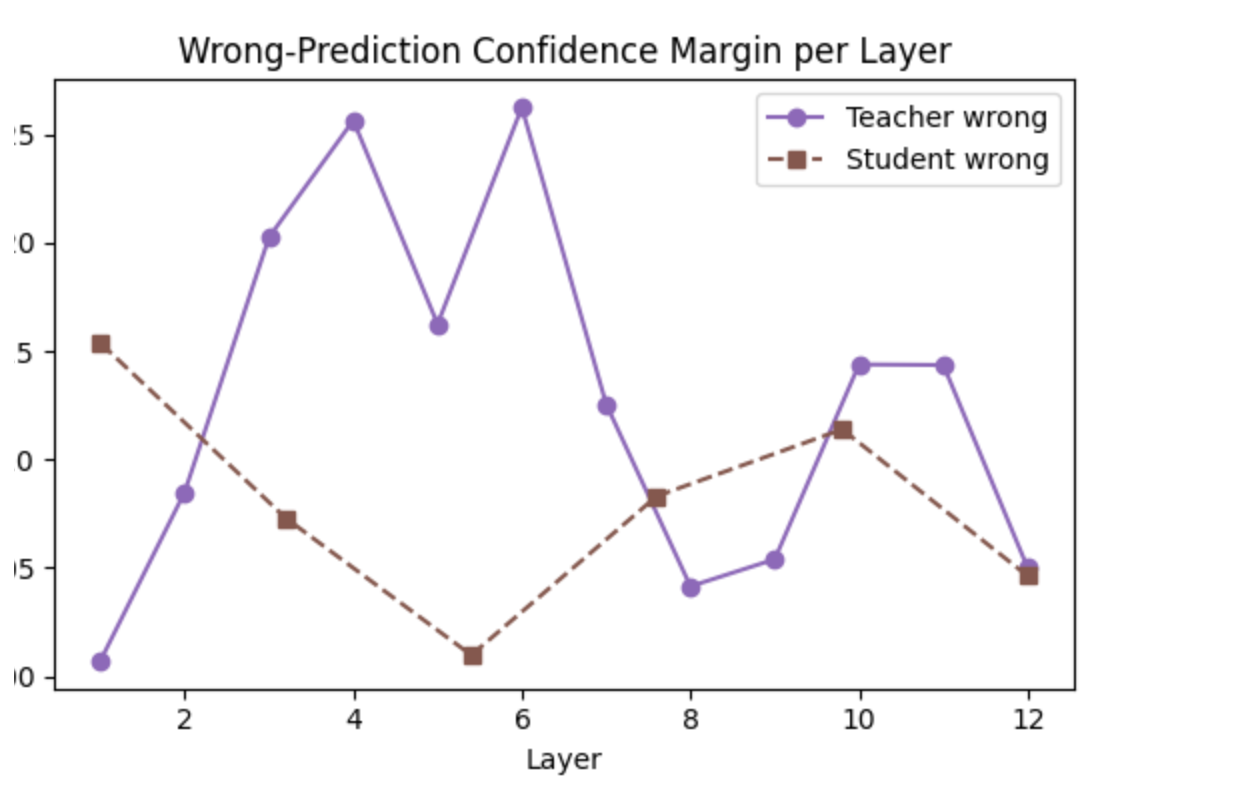
\includegraphics[width=\linewidth]{figs/aux_3_wrong.png}
                \caption{Auxiliary network on layer 3}
                \label{fig:aux3}
            \end{subfigure}
            \hfill
            \begin{subfigure}[t]{0.45\linewidth}
                \centering
                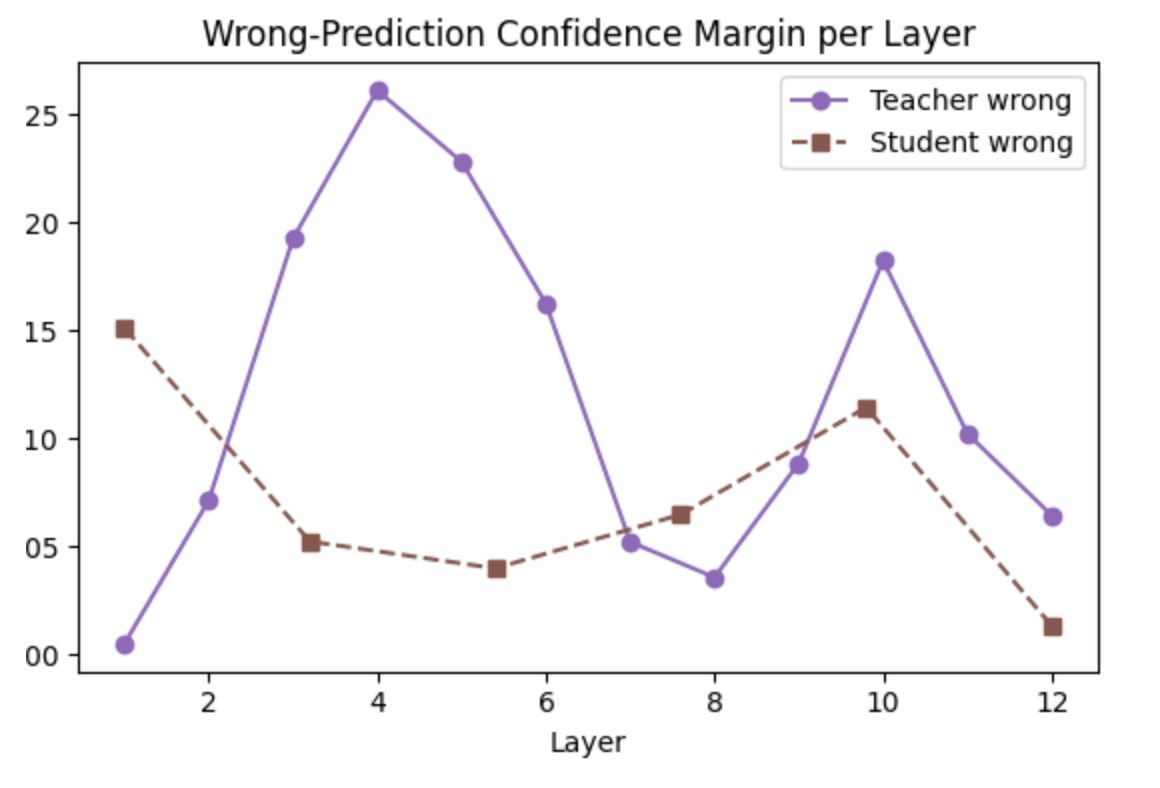
\includegraphics[width=\linewidth]{figs/aux_6_wrong.png}
                \caption{Auxiliary network on layer 6 (last layer)}
                \label{fig:aux6}
            \end{subfigure}
            \caption{Confidence margins in student and teacher on the predictions that were wrong}
            \label{fig:wrong-pred-con}
        \end{figure}
    }

\end{frame}

\section{Analysis And Future Work}
\begin{frame}{Analysis And Future Work}
    \begin{itemize}
        \item Minor improvement in accuracy of the student model by the proposed approach over DEDIER on MultiNLI
        \item Still more testing needed, on varied datasets and teacher models for justifying its use.
        \item The confidence margins are generally lower than one used in DEDIER work.
        \item Need to study effects of increasing layers of Aux network
        \item Hyperparameter tuning 
    \end{itemize}
\end{frame}
\begin{frame}{Conclusion}
    \begin{itemize}
        \item Cheap, effective uncertainty via Laplace in early exits.
        \item Uncertainty reweights KD loss in student models.
        \item Reduces reliance on simple features.
    \end{itemize}
\end{frame}


% \againframe<3-4>{slide:KD}
% \item<2-> Smaller Student model that mimics larger teacher model that generalises well
% \item<3-> The negative examples give info about dataset that is not captured by the cross entropy loss
% \item<4-> Teacher Provides "Soft Targets"
% \item<5-> minimise the kl divergence of last layer logits of the teacher along with cross entropy loss
% \begin{tikzpicture}<1>
%     \node at (0,0){Text Test};
% \end{tikzpicture}

\begin{frame}{References}
    \footnotesize
    %  \bibliography{reference.bib}
    \bibliographystyle{apalike}
    \bibliography{optML.bib}
\end{frame}

\end{document}
